\documentclass[letterpaper, 10pt, conference, twoside]{ieeeconf}


\IEEEoverridecommandlockouts
\overrideIEEEmargins
\usepackage{ctex}
\usepackage{booktabs}
\usepackage{graphicx}
\graphicspath{{figures/}}%图片所在的目录

\usepackage{lastpage}%获得总页数
\usepackage{fancyhdr}
\pagestyle{fancy}
%以下命令中L--左侧 R--右侧 C--中间 O--奇数页 E--偶数页
%\fancyhead[LO,RE]{机器学习原理、工程技术与应用}%奇数页左侧,偶数页右侧显示页眉
\fancyhead[CO,RE]{机器学习}%奇数页左侧,偶数页右侧显示页眉
\fancyhead[LO,CE]{代课教师 李乡儒,华南师范大学计算机学院}%奇数页左侧,偶数页中间页脚为空
\fancyhead[RO,LE]{\today}%奇数页右侧,偶数页左侧显示 当前页 of 总页数
\fancyfoot[CO,RE]{机器学习}%奇数页中间,偶数页右侧页脚为空
\fancyfoot[LO,CE]{2021-2022-2学期}%奇数页左侧,偶数页中间页脚为空
\fancyfoot[RO,LE]{\thepage\ of \pageref{LastPage}}%奇数页右侧,偶数页左侧显示 当前页 of 总页数
\renewcommand{\headrulewidth}{0.4pt}%改为0pt即可去掉页眉下面的横线
\renewcommand{\footrulewidth}{0.4pt}%改为0pt即可去掉页脚上面的横线
\setlength{\voffset}{-10mm}
\setlength{\topmargin}{0mm}
\setlength{\headheight}{5mm}
\setlength{\headsep}{5mm}
\setlength{\footskip}{8mm}



\title{\LARGE \bf
基于U-Net的胃肠道图像分割
}


\author{2021023206 \quad 徐力\\ \today\\ 机器学习课程作业}

\usepackage{makecell}

\begin{document}

\maketitle
%\thispagestyle{empty}
%\pagestyle{empty}



\begin{abstract}
该模板适用于机器学习高级技术及应用课程. 所有地方使用英文状态下的标点符号, 标点符号之后空一个空格.

\vspace{1ex}\noindent\textbf{关键词}: 词1; 词2

\end{abstract}

\begin{eabstract}
	English Abstract
	
\vspace{1ex}\noindent\textbf{Keywords}: word1; word2
\end{eabstract}


\section{引言}
医学图像分割是医学图像处理与分析领域的复杂而关键的步骤,其目的是将医学图像中具有某些特殊含义的部分分割出来,并提取相关特征,为临床诊疗和病理学研究提供可靠的依据,辅助医生作出更为准确的诊断。 医学图像具有复杂性,在分割过程中需要解决不均匀及个体差异等一系列问题,所以一般的图像分割方法难以直接应用于医学图像分割。

UW-Madison 胃肠道图像分割(UW-Madison GI Tract Image Segmentation)是一场研究型代码竞赛,要求在医学扫描中跟踪健康肠胃器官的准确位置以改善肠胃癌的放射治疗。在治疗当中,借助集成磁共振成像和线性加速器系统(也称为 MR-Linacs)等技术,为了指向肿瘤施加高剂量辐射,同时避开肠和胃,放射肿瘤学家必须手动勾勒出胃和肠的位置。这项工作非常耗时,因为肿瘤、肠和胃的位置每天都在变化,使得治疗时间大大延长。

在比赛中,需要创建模型以在MRI扫描中自动分割肠和胃。在给出的数据集中,不同的患者在不同日子里进行了多次MRI扫描,每次扫描包括多张断层扫描。
% \subsection{二级标题}
% \subsubsection{三级标题}

\section{U-Net框架}
U-Net 的构建基于“全卷积网络”。它由收缩路径(左侧)和扩展路径(右侧)组成。收缩路径遵循卷积网络的典型架构。它由两个 3x3 卷积(未填充卷积)的重复应用组成,每个卷积后跟一个整流线性单元 (ReLU) 和一个 2x2 最大池化操作,步幅为 2,用于下采样。在每个下采样步骤中,我们将特征通道的数量加倍。扩展路径中的每一步都包括对特征图进行上采样,然后是将特征通道数量减半的 2x2 卷积(“上卷积”),与收缩路径中相应裁剪的特征图的连接,以及两个 3x3卷积,每个后跟一个 ReLU。由于在每个卷积中都会丢失边界像素,因此收缩路径中的图像需要经过裁剪,再与扩展路径中相应的图像拼接。在最后一层,使用 1x1 卷积将每个 64 分量特征向量映射到所需数量的类。该网络总共有 23 个卷积层,如图 1 所示。
\begin{figure}[htbp]
  \centering
  \includegraphics[width = 1\linewidth]{structure.png}
  \caption{U-Net 结构}
  \label{fig:fig1}
\end{figure}

在上采样部分,上采样的特征图包含了上下文信息,并与来自收缩路径的高分辨率特征结合,将上下文信息传播到更高分辨率的层。分割图只包含输入图像中完整上下文可用的像素,为了预测图像边界区域中的像素,通过镜像输入图像来推断缺失的上下文,如图2所示。

\begin{figure}[htbp]
  \centering
  \includegraphics[width = 1\linewidth]{seamless-seg.png}
  \caption{镜像拼接原图,以补充边缘像素缺失的上下文}
  \label{fig:fig2}
\end{figure}

生物医学图像分割中,可用的训练数据通常较少。因此,需要对可用的训练图像应用数据增强,如弹性变形等。这允许网络学习对此类变形的不变性。同时在生物医学当中,变形曾经是组织中最常见的变化,并且可以有效地模拟真实的变形。通过数据增强,模型学习数据的不变性特征,从而防止过拟合。


\section{赛题数据分析}

竞赛给出16位灰度 PNG 图像,参赛者需要在图像中分割器官细胞。训练注释以 RLE 编码掩码的形式提供。

比赛中有多个病例,每个病例的扫描分为多组,每组由扫描发生的日期标识,扫描的当天产生多张扫描切片。一部分病例按照扫描日期的先后划分为训练集和测试集;另外一部分病例的全部数据处于训练集或测试集中。因此,模型不仅需要针对见过的病例标注其器官位置,也需要标注完全没见过的病例。

训练集中,每个病例的扫描次数(天数)在1到6之间。

\begin{table}[htbp]
  \centering
 \caption{数据集的统计数据}
 \label{tab:table1}
 \begin{tabular}{llll}
  \toprule
  \makecell[l]{注释数量\\(图片数量)} & 病例数量 & \makecell[l]{无掩码\\图片数量}& \makecell[l]{有掩码\\图片数量}\\
  \midrule
    38496&85&21906&16590\\
  \bottomrule
 \end{tabular}
\end{table}

\begin{table}[htbp]
  \centering
 \caption{扫描次数统计}
 \label{tab:table2}
 \begin{tabular}{l|ccccccc}
  \toprule
  \makecell[l]{扫描\\次数}& 1次 & 2次 & 3次 & 4次 & 5次 & 6次 & 合计\\
  \midrule
  \makecell[l]{病例\\数量}& 9 & 8 & 45 & 2 & 20 & 1 & 85\\
  \bottomrule
 \end{tabular}
\end{table}

\begin{table}[htbp]
  \centering
  \caption{胃、大肠和小肠的共现;其中对角线上的数字表示该器官的总出现次数}
  \label{tab:table3}
\begin{tabular}{||c||c|c|c||}
\hline
次数&胃&大肠&小肠 \\
\hline\hline
胃&8627&6181&3361 \\
\hline
大肠&6181&14085&10982 \\
\hline
小肠&3361&10982&11201 \\
\hline
\end{tabular}
\end{table}


\begin{figure}[htbp]
  \centering
  \includegraphics[width = 1\linewidth]{nseg-per-img.png}
  \caption{每张图片的分割掩码数量}
  \label{fig:fig3}
\end{figure}

如表1所示,数据集中一共有38496张图片,其中没有掩码的图片有21906张,占56.9046\%;有至少一类掩码的图片有16590张,占43.0954\%。这些扫描图片来自一共85个病例。

每个病例的扫描次数(天数)在1次(天)到6次(天)之间,如表2所示。其中,最多的病例(45例)是扫描了3次,其次(20例)是扫描了5次。按照比赛规则,部分病例的不同阶段的扫描被分别划分到了训练集和测试集,这可能是扫描次数分布不规律的原因。

进一步统计当图片的掩码分别存在0、1、2、3类时对应的各器官种类的数量,如图3所示。没有注释的情况可在表1中观察,下面分别观察图片存在1、2、3种掩码的情况:

\subsection{存在一种掩码的图片}
存在且仅存在一种掩码的图片一共有2468张,占6.41\%。在这些注释当中,大多数的注释是关于胃。其中,胃的注释有2286个,占92.6\%;大肠的注释有123个,占4.98\%;小肠的注释有59个,仅占2.39\%。

\subsection{存在两种掩码的图片}
存在且仅存在两种掩码的图片一共有10921张,占28.37\%.在这些注释当中,大多数的注释的组合是关于大肠和小肠。其中,大肠-小肠的注释有7781个,占71.3\%;大肠-胃的注释有2980个,占27.3\%;小肠-胃的注释有160个,仅占1.47\%。

\subsection{存在三种掩码的图片}
存在三种掩码的图片一共有3201张,占8.32\%.

如表3所示。所有注释一共有33913条,其中最多的种类是大肠(14085条),其次是小肠(11201条)、胃(8627条),分别占41.53\%,33.03\%,25.44\%.一次共现在这里表示为一对注释在同一张扫描图片上同时出现。胃-大肠、大肠-小肠、小肠-胃的共现分别是6181、10982、3361。可见,断层扫描图片中,最常同时出现器官的是大肠和小肠,最少同时出现的是小肠和胃。造成的原因可能是身体结构导致的器官分布规律:大肠通常分布在胃的下方,而小肠分布在大肠的下方。

数据集中的图片尺寸主要有(266,266)和(310,360)两种,此外还有(276,276)和(234,234),如表4所示。

\begin{table}[htbp]
  \centering
  \caption{不同尺寸的图片数量}
  \label{tab:table4}
  \begin{tabular}{cccc|c}
    \toprule
    (266,266)&(310,360)&(276,276)&(234,234)&合计 \\
    \midrule
      25920&11232&1200&144&38496\\
    \bottomrule
   \end{tabular}
\end{table}

数据集注释采用游程编码(RLE, run-length encoding)格式。每个像素可以属于背景,或大肠、小肠、胃当中的一类或多类。典型掩码标签的可视化如图4所示。部分器官分割注释是有重叠的,如图5所示,有一部分大肠的注释完全处于小肠的注释当中。因此本竞赛是逐个像素的多标签多分类任务。

\begin{figure}[htbp]
  \centering
  \includegraphics[width = 1\linewidth]{seg_view.png}
  \caption{典型的掩码标签注释}
  \label{fig:fig4}
\end{figure}

\begin{figure}[htbp]
  \centering
  \includegraphics[width = 1\linewidth]{seg_overlay.png}
  \caption{重叠的掩码标签注释}
  \label{fig:fig5}
\end{figure}

为了进一步探究将竞赛作为单标签多分类处理会造成的损失,统计不同种类和不同大小的掩码重叠发生的次数,如图6所示。胃-大肠-小肠重叠掩码的面积可达到300以上;大肠-小肠重叠掩码的面积可达到600以上。因此,掩码应表示为$W\times H\times 3$。其中3个通道分别表示不同的掩码类型。

对于给定的病例和扫描天数为单次扫描。单次扫描得到一系列连续的断层切片,得到的切片数量有两种情况:144张或80张。一共259次扫描是144张,15次扫描是80张。统计所有不同位置的切片包含器官掩码的数量,分布近似钟形曲线,如图7所示。观察得到,胃、大肠、小肠在扫描切片上分布达到峰值所在的位置分别为67、100、102,对应的最大注释数量分别为196、240、235个。大肠和小肠对峰值以左的切片位置有所偏置,而胃有向右的偏置。小肠、胃的扫描切片位置相对大肠较为集中。可见,器官扫描切片数量峰值的位置排序符合器官的大致高低位置排序(胃>大肠>小肠);而峰值的注释数量排序符合各器官总注释数量的排序(大肠>小肠>胃)。

\begin{figure}[htbp]
  \centering
  \includegraphics[width = 1\linewidth]{seg_overlay_distribution.png}
  \caption{分割掩码重叠面积的分布}
  \label{fig:fig6}
\end{figure}

\begin{figure}[htbp]
  \centering
  \includegraphics[width = 1\linewidth]{seg_distribution.png}
  \caption{分割掩码重叠面积的分布}
  \label{fig:fig7}
\end{figure}

\section{实验}
\subsection{评价指标}
\subsubsection{三级标题}

\subsection{实验设置}

\subsection{结果分析}

\section{结论}
\subsection{二级标题}
\subsubsection{三级标题}

\section{图表}

\begin{figure}[htbp]
  \centering
  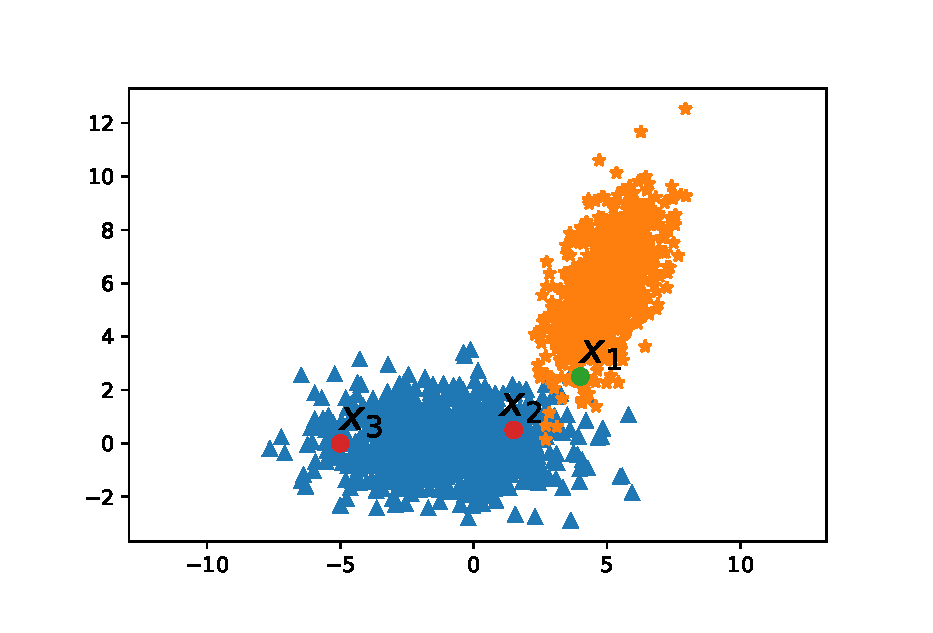
\includegraphics[width = 1\linewidth]{smooth}
  \caption{图片名称及图片内容简介}
  \label{fig:fig2}
\end{figure}


\begin{table}[htbp]
  \centering
 \caption{三线表}
 \label{tab:table2}
 \begin{tabular}{llll}
  \toprule
  表头1 & 表头2 & 表头3& 表头4\\
  \midrule
    模&式&识&别\\
    机&器&学&习\\
    数&据&挖&掘\\
    人&工&智&能\\
  \bottomrule
 \end{tabular}
\end{table}




\section{列点}

\begin{itemize}
\item The word ÒdataÓ is plural, not singular.
\item The subscript for the permeability of vacuum ?0, and other common scientific constants, is zero with subscript formatting, not a lowercase letter ÒoÓ.
\end{itemize}

\begin{enumerate}
\item The word ÒdataÓ is plural, not singular.
\item The subscript for the permeability of vacuum ?0, and other common scientific constants, is zero with subscript formatting, not a lowercase letter ÒoÓ.
\end{enumerate}


\section{脚注}
机器学习\footnote{脚注内容}

\section{列点}

\begin{itemize}
\item The word ÒdataÓ is plural, not singular.
\item The subscript for the permeability of vacuum ?0, and other common scientific constants, is zero with subscript formatting, not a lowercase letter ÒoÓ.
\end{itemize}

\begin{enumerate}
\item The word ÒdataÓ is plural, not singular.
\item The subscript for the permeability of vacuum ?0, and other common scientific constants, is zero with subscript formatting, not a lowercase letter ÒoÓ.
\end{enumerate}


\section{列点}

\begin{itemize}
\item The word ÒdataÓ is plural, not singular.
\item The subscript for the permeability of vacuum ?0, and other common scientific constants, is zero with subscript formatting, not a lowercase letter ÒoÓ.
\end{itemize}

\begin{enumerate}
\item The word ÒdataÓ is plural, not singular.
\item The subscript for the permeability of vacuum ?0, and other common scientific constants, is zero with subscript formatting, not a lowercase letter ÒoÓ.
\end{enumerate}


\section{列点}

\begin{itemize}
\item The word ÒdataÓ is plural, not singular.
\item The subscript for the permeability of vacuum ?0, and other common scientific constants, is zero with subscript formatting, not a lowercase letter ÒoÓ.
\end{itemize}

\begin{enumerate}
\item The word ÒdataÓ is plural, not singular.
\item The subscript for the permeability of vacuum ?0, and other common scientific constants, is zero with subscript formatting, not a lowercase letter ÒoÓ.
\end{enumerate}


\section{列点}

\begin{itemize}
\item The word ÒdataÓ is plural, not singular.
\item The subscript for the permeability of vacuum ?0, and other common scientific constants, is zero with subscript formatting, not a lowercase letter ÒoÓ.
\end{itemize}

\begin{enumerate}
\item The word ÒdataÓ is plural, not singular.
\item The subscript for the permeability of vacuum ?0, and other common scientific constants, is zero with subscript formatting, not a lowercase letter ÒoÓ.
\end{enumerate}

\section{列点}

\begin{itemize}
\item The word ÒdataÓ is plural, not singular.
\item The subscript for the permeability of vacuum ?0, and other common scientific constants, is zero with subscript formatting, not a lowercase letter ÒoÓ.
\end{itemize}

\begin{enumerate}
\item The word ÒdataÓ is plural, not singular.
\item The subscript for the permeability of vacuum ?0, and other common scientific constants, is zero with subscript formatting, not a lowercase letter ÒoÓ.
\end{enumerate}


\section{列点}

\begin{itemize}
\item The word ÒdataÓ is plural, not singular.
\item The subscript for the permeability of vacuum ?0, and other common scientific constants, is zero with subscript formatting, not a lowercase letter ÒoÓ.
\end{itemize}

\begin{enumerate}
\item The word ÒdataÓ is plural, not singular.
\item The subscript for the permeability of vacuum ?0, and other common scientific constants, is zero with subscript formatting, not a lowercase letter ÒoÓ.
\end{enumerate}

\section{列点}

\begin{itemize}
\item The word ÒdataÓ is plural, not singular.
\item The subscript for the permeability of vacuum ?0, and other common scientific constants, is zero with subscript formatting, not a lowercase letter ÒoÓ.
\end{itemize}

\begin{enumerate}
\item The word ÒdataÓ is plural, not singular.
\item The subscript for the permeability of vacuum ?0, and other common scientific constants, is zero with subscript formatting, not a lowercase letter ÒoÓ.
\end{enumerate}

\section{列点}

\begin{itemize}
\item The word ÒdataÓ is plural, not singular.
\item The subscript for the permeability of vacuum ?0, and other common scientific constants, is zero with subscript formatting, not a lowercase letter ÒoÓ.
\end{itemize}

\begin{enumerate}
\item The word ÒdataÓ is plural, not singular.
\item The subscript for the permeability of vacuum ?0, and other common scientific constants, is zero with subscript formatting, not a lowercase letter ÒoÓ.
\end{enumerate}

\section{列点}

\begin{itemize}
\item The word ÒdataÓ is plural, not singular.
\item The subscript for the permeability of vacuum ?0, and other common scientific constants, is zero with subscript formatting, not a lowercase letter ÒoÓ.
\end{itemize}

\begin{enumerate}
\item The word ÒdataÓ is plural, not singular.
\item The subscript for the permeability of vacuum ?0, and other common scientific constants, is zero with subscript formatting, not a lowercase letter ÒoÓ.
\end{enumerate}

\section{列点}

\begin{itemize}
\item The word ÒdataÓ is plural, not singular.
\item The subscript for the permeability of vacuum ?0, and other common scientific constants, is zero with subscript formatting, not a lowercase letter ÒoÓ.
\end{itemize}

\begin{enumerate}
\item The word ÒdataÓ is plural, not singular.
\item The subscript for the permeability of vacuum ?0, and other common scientific constants, is zero with subscript formatting, not a lowercase letter ÒoÓ.
\end{enumerate}

\section{列点}

\begin{itemize}
\item The word ÒdataÓ is plural, not singular.
\item The subscript for the permeability of vacuum ?0, and other common scientific constants, is zero with subscript formatting, not a lowercase letter ÒoÓ.
\end{itemize}

\begin{enumerate}
\item The word ÒdataÓ is plural, not singular.
\item The subscript for the permeability of vacuum ?0, and other common scientific constants, is zero with subscript formatting, not a lowercase letter ÒoÓ.
\end{enumerate}

\section{列点}

\begin{itemize}
\item The word ÒdataÓ is plural, not singular.
\item The subscript for the permeability of vacuum ?0, and other common scientific constants, is zero with subscript formatting, not a lowercase letter ÒoÓ.
\end{itemize}

\begin{enumerate}
\item The word ÒdataÓ is plural, not singular.
\item The subscript for the permeability of vacuum ?0, and other common scientific constants, is zero with subscript formatting, not a lowercase letter ÒoÓ.
\end{enumerate}


\begin{thebibliography}{99}

\bibitem{c1} G. O. Young, ÒSynthetic structure of industrial plastics (Book style with paper title and editor),Ó 	in Plastics, 2nd ed. vol. 3, J. Peters, Ed.  New York: McGraw-Hill, 1964, pp. 15Ð64.
\bibitem{c2} W.-K. Chen, Linear Networks and Systems (Book style).	Belmont, CA: Wadsworth, 1993, pp. 123Ð135.

\end{thebibliography}
\end{document}
